\documentclass{article}
\usepackage{tikz}
\usepackage[paperwidth=9.5cm, paperheight=5.7cm,left=0pt,right=0pt,top=2pt,bottom=2pt]{geometry}
\begin{document}
\centering
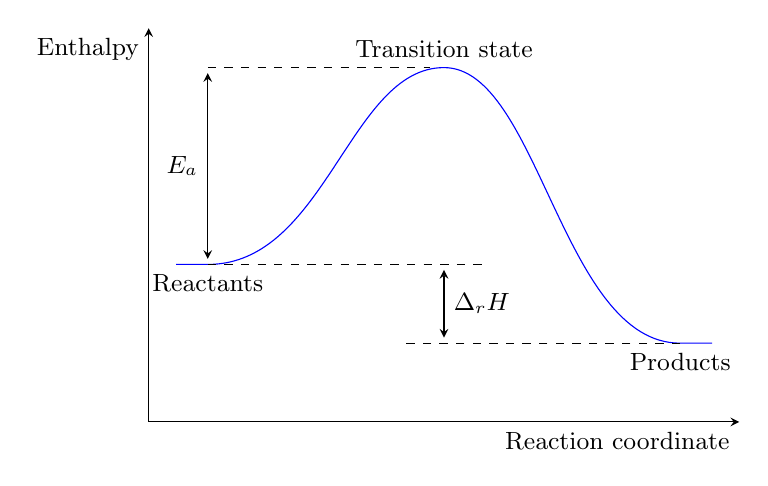
\begin{tikzpicture}[x=1.5cm, every node/.append style={font=\small}]
% axis
\draw[-stealth] (0,0) -- (0,5) node[below left] {Enthalpy};
\draw[-stealth] (0,0) -- (5,0) node[below left] {Reaction coordinate};

% molecules
\node[below] (reac)       at (0.5,2)   {Reactants};
\node[above] (transState) at (2.5,4.5) {Transition state};
\node[below] (prod)       at (4.5,1)   {Products};

% reaction path
\draw[blue] (reac.150) -- (reac.north) .. controls ++(1,0) and ++(-0.8,0) .. (transState.south) .. controls ++(0.8,0) and ++(-1,0) .. (prod.north) -- (prod.30);

% activation energy
\draw[shorten >=2pt, shorten <=2pt, stealth-stealth] (reac.north) -- (reac.north |- transState.south) node[pos=0.5,left]{$E_a$};
\draw[shorten >=5pt, dashed] (reac.north |- transState.south) -- (transState.south);

% reaction enthalpy
\draw[shorten >=5pt, dashed] (reac.north) -- ++(2.5,0);
\draw[shorten >=5pt, dashed] (prod.north) -- ++(-2.5,0);
\draw[shorten >=2pt, shorten <=2pt,stealth-stealth] (reac.north -| transState) -- (prod.north -| transState) node[pos=0.5,right] {$\Delta_rH$};

\end{tikzpicture}
\end{document}
